\chapterimage{CCD.jpg} % Chapter heading image

\chapter{Detektorji svetlobe}

V tem poglavju bomo spoznali detektorje svetlobe, ki so nujni za kvantitativno obravnavo
optičnih pojavov in sprejemanje optičnih signalov. Detektorji\index{Detektor}
se med seboj razlikujejo po načinu delovanja in po svojih specifikacijah, 
ki jih bomo podrobneje spoznali v nadaljevanju. Največ
pozornosti bomo posvetili polprevodniškim detektorjem, ki so danes najbolj razširjeni.
Na koncu bomo spoznali še šum pri detekciji, ki omejuje uporabnost naprav.

\section{Osnovne karakteristike detektorjev}
Osnovna naloga optičnih detektorjev je spremeniti vpadni svetlobni signal 
v nek drug signal, ki ga lahko natančno merimo. Navadno sta to električni tok 
ali električna napetost, ki pa sta sorazmerna z močjo vpadne svetlobe 
in ne z amplitudo električne poljske jakosti. Pri navadni detekciji se tako
podatek o fazi valovanja izgubi. V grobem delimo detektorje v dve skupini, 
na termične\index{Detektor!termični} in kvantne\index{Detektor!kvantni}. 
Prvi pretvorijo energijo vpadne svetlobe v toploto, drugi pa temeljijo na 
fotoefektu\index{Fotoefekt}, pri katerem vpadli foton iz snovi izbije 
elektron ali v snovi ustvari par elektron--vrzel.

Termični detektorji zaznavajo svetlobo preko povišanja temperature 
senzorja zaradi absorbirane svetlobe. Taki detektorji zaznavajo energijo 
vpadle svetlobe. Njihov odziv je razmeroma počasen, zato jih uporabljamo
predvsem za merjenje optične moči, lahko tudi zelo velike. Po drugi strani pa je odziv
termičnih detektorjev neodvisen
od valovne dolžine vpadne svetlobe, zaradi česar so termični detektorji uporabni na 
širokem območju od globoke ultravijolične do daljne infrardeče svetlobe. 
\index{Ultravijolično valovanje}\index{Infrardeče valovanje}Uporaba
prevlada predvsem v infrardrečem, teraherčnem ali celo mikrovalovnem območju, kjer so 
drugi detektorji bistveno manj občutljivi. \index{Teraherčno valovanje}
Primeri termičnih detektorjev so bolometer, termočlen in piroelektrični detektor.
\index{Bolometer}\index{Termočlen}\index{Piroelektrični detektor}

Druga skupina so kvantni detektorji, v katerih se
fotoni absorbirajo in povzročijo pojav prostih nosilcev naboja. Taki detektorji
zaznavajo število vpadlih fotonov. Odlikuje jih zelo hiter odziv 
(tipično pod $\si{\micro\second}$)
in velika občutljivost. Njihova poglavitna slabost je omejen obseg valovnih dolžin,
pri katerih zaznavajo svetlobo, poleg tega jih je za optimalno delovanje treba 
hladiti. Primeri so vakuumske, polprevodniške in plazovne fotodiode.
\index{Fotodioda!vakuumska}\index{Fotodioda!polprevodniška}\index{Fotodioda!plazovna}
\begin{figure}[h]
\centering
\def\svgwidth{65truemm} 
\input{slike/11_ShemaTermKv.pdf_tex}
\caption{Primerjava spektralnega odziva termičnega in kvantnega detektorja}
\label{fig:shemaTermKv}
\end{figure}

Osnovne karakteristike, ki omogočajo primerjavo detektorjev in določajo njihovo uporabnost,
so občutljivost, spektralni odziv, odzivni čas in prag detekcije. 
\index{Detektor!občutljivost}
\index{Detektor!spektralni odziv}
\index{Detektor!odzivni čas}
\index{Detektor!prag detekcije}

\begin{enumerate}
\item Občutljivost $R$ pove, koliko je izhodnega signala 
na enoto vpadnega svetlobnega toka. Enota za občutljivost je A/W, če merimo tok, ali V/W, 
če na izhodu zaznavamo napetost. 
\item Spektralni odziv pove, kako se občutljivost spreminja z valovno dolžino $R(\lambda)$.
Pri termičnih detektorjih je $R(\lambda)$ konstanta, medtem ko kvantni detektorji 
delujejo le v določenem območju valovnih dolžin, ki je odvisen od snovi, 
iz katere je detektor narejen. 
\item Odzivni čas pove, kako hitro se detektor odzove na spremembo optičnega signala. Predvsem 
optične telekomunikacije zahtevajo izredno hiter odziv.
\item Prag detekcije pove, pri kolikšni vpadni svetlobni moči postane razmerje med signalom ($S$)
in šumom ($N$, {\it noise}) enako $S/N = 1$. \index{Razmerje signal proti šumu}
\end{enumerate}

\section{Termični detektorji}
\index{Detektor!termični}
Termične detektorje se zaradi njihovega razmeroma počasnega odziva uporablja predvsem 
za merjenje vpadne moči in za detekcijo svetlobe tistih valovnih dolžin, za katere 
ni drugih preprostih ali učinkovitih detektorjev. Pogosto se uporabljajo za termografske 
kamere in v astronomiji.

Delovanje termičnih detektorjev temelji na spremembi temperature zaradi absorpcije svetlobe 
(energije). Detektorji se med seboj razlikujejo predvsem v načinu pretvorbe spremembe 
temperature v električni signal.\index{Absorpcija}
Tipalo termičnih detektorjev mora biti pri vseh vrstah dobro počrnjeno, da absorbira
svetlobo v čim širšem spektralnem območju. Čeprav je njihova občutljivost načeloma 
neodvisna od valovne dolžine vpadne svetlobe, se v praksi pojavijo omejitve zaradi
prepustnosti okna in absorpcijskega spektra črnega nanosa. Tipala so majhna, zato 
da dosežemo čim hitrejši odziv, ki pa je kljub temu navadno počasnejši od $1~\si{ms}$. 
Sodobnejši detektorji se po odzivnem času že približujejo 
kvantnim, saj dosegajo odzivne čase tudi do $\sim 10~\si{\micro\second}$. 
Termične detektorje uporabljamo pri sobni temperaturi,  
za zahtevne meritve pa jih hladimo na nekaj $\si{K}$. 

Obravnavajmo termični detektor, katerega tipalo naj ima toplotno kapaciteto $C$. Toplota
se s tipala odvaja v nek toplotni zalogovnik s temperaturo $T_0$, 
toplotne izgube pa označimo z $\Lambda$. Ko na tipalo vpada svetloba z močjo $P$, 
začne temperatura tipala $T$ zaradi absorpcije svetlobe naraščati, hkrati pa se tipalo 
ohlaja zaradi odtekanja toplote. Zapišemo
\begin{equation}
\frac{dW}{dt} = C \frac{dT}{dt} = P - \Lambda (T-T_0).
\label{TD1}
\end{equation}
V stacionarnem stanju (ob konstantnem vpadnem svetlobnem toku) se
temperatura tipala ne spreminja in razlika temperature tipala in zalogovnika je 
\begin{equation}
T - T_0 = \frac{P}{\Lambda}.
\label{temp_sens}
\end{equation}
Občutljivost detektorja, ki je sorazmerna z razliko temperatur, 
je torej obratno sorazmerna s toplotnimi izgubami. Za večjo občutljivost moramo
toplotne izgube detektorja kar se da zmanjšati. 

Po enačbi~(\ref{TD1}) se temperatura približuje stacionarni vrednosti s časovno konstanto 
\begin{equation}
\tau = \frac{C}{\Lambda},
\label{TermD_t}
\end{equation}
ki je ključni parameter za določanje odzivnega časa detektorja. Odzivni
čas je sorazmeren s kapaciteto senzorja, zato so tipala praviloma 
zelo majhna.\index{Detektor!odzivni čas}

Iz enačbe~(\ref{TermD_t}) sledi, da moramo za dosego čim krajšega odzivnega časa toplotne izgube 
kar se da povečati. Velike izgube sicer skrajšajo odzivni čas, 
vendar tudi zmanjšajo občutljivost (enačba~\ref{temp_sens}), 
zato termični detektorji ne morejo imeti hkrati velikega in hitrega odziva. 
Če želimo toplotne izgube povečati in s tem skrajšati odzivni čas, detektorje hladimo z zrakom 
ali celo z vodo, majhne toplotne izgube pa so omejene s sevanjem.  

Podrobneje poglejmo odziv termičnega detektorja od vpadne moči. Naj se vpadna moč
spreminja s časom, temperatura na detektorju pa temu sledi z določeno zakasnitvijo. Odziv
najlepše izračunamo v Fourierevem prostoru. Vpadno moč in temperaturo izrazimo kot
\begin{equation}
P(t) = \int_{-\infty}^{\infty} P_\omega e^{i\omega t}d\omega \quad \mathrm{in} \quad
T = T_0 + \int_{-\infty}^{\infty} T_\omega e^{i\omega t}d\omega.
\label{TermTF}
\end{equation}
To vstavimo v enačbo~(\ref{TD1}) in zapišemo
\begin{equation}
\int_{-\infty}^{\infty} i \omega T_\omega e^{i\omega t}d\omega = \frac{1}{C}
\int_{-\infty}^{\infty} (P_\omega - \Lambda T_\omega) e^{i\omega t}d\omega.
\end{equation}
Enačbi zadostimo, če izenačimo člene pred vsako spektralno komponento posebej
\begin{equation}
i \omega T_\omega = \frac{1}{C}\left(P_\omega - \Lambda T_\omega\right).
\end{equation}
Če vpeljemo odzivni čas $\tau$ (enačba~\ref{TermD_t}), \index{Detektor!odzivni čas}sledi
\begin{equation}
T_\omega = \frac{1}{\Lambda}\left(\frac{1}{1+i \omega \tau}\right)P_\omega.
\label{TermOdziv}
\end{equation}
Tako smo tudi z računom pokazali, da detektor sledi le počasnim spremembam signala. 
\begin{definition}
Pokaži, da je odziv termičnega detektorja na zelo kratek svetlobni sunek oblike 
$P(t) = P_0 \delta(t-t_0)$ enak 
\begin{equation}
T(t)=\frac{iP_0}{\Lambda}e^{-(t-t_0)/\tau}.
\end{equation}
\end{definition}

\subsection*{Bolometer}
Bolometer je termični detektor\index{Bolometer}, pri katerem zaznavamo spremembo 
električne upornosti
zaradi spremembe temperature tipala\footnote{Prvi bolometer je leta 1881 naredil
ameriški fizik, astronom in letalski inženir Samuel Pierpont Langley, 1834--1906.}. 
Tipalo je praviloma počrnjena tanka ploščica, 
navadno je narejena iz termistorja\footnote{Termistor je upornik, katerega
upornost se spreminja s temperaturo.}, \index{Termistor}
polprevodnika ali superprevodnika. Tipalo preko
referenčnega upora priključimo na napetost, preko kondenzatorja pa merimo napetost na njem.
Za meritve konstantega svetlobnega toka tipalo navadno vežemo v Wheatstonov mostiček. V obeh
primerih za referenčni upor vzamemo enako tipalo, ki pa ga zaščitimo pred vpadno svetlobo, 
tako da postane sistem neobčutljiv na morebitne spremembe temperature okolice.
\begin{figure}[h!]
\centering
\def\svgwidth{75truemm} 
\input{slike/11_bolometer.pdf_tex}
\caption{Shema bolometra}
\label{fig:Bolometer-shema}
\end{figure}

Prednost bolometrov s termistorjem je približno linearna zveza med upornostjo in 
temperaturo. Uporabljamo jih predvsem za merjenje večjih vpadnih moči, saj taki 
detektorji niso zelo občutljivi ($R\sim 100~\si{\volt/\watt}$). 
So pa robustni, stabilni in delujejo pri sobni 
temperaturi. Odzivni časi so okoli $\tau \sim 1$--$20~\si{\milli\second}$. 
Pri polprevodniških bolometrih upornost pojema eksponentno s temperaturo. 
Primerni so za detekcijo teraherčnih valovanj,\index{Teraherčno valovanje} 
vendar mora biti za ta namen 
bolometer (npr. germanijev) hlajen s tekočim helijem. Tako lahko dosežemo
občutljivosti večje od $R \sim 10^8~\si{\volt/\watt}$. Zelo občutljivi so tudi 
detektorji s superprevodnimi tipali, saj je odvisnost upornosti od temperature v bližini
prehoda v superprevodno stanje zelo velika ($R \sim 10^3~\si{\volt/\watt}$).

\begin{figure}[h]
\centering
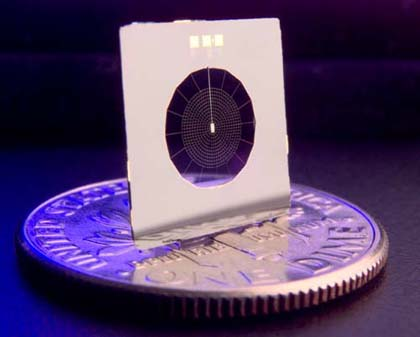
\includegraphics[width=75truemm]{slike/11_Bolometer.jpg}
\caption{Bolometer za merjenje prasevanja. Premer kovanca za primerjavo je 18~mm. 
Vir: NASA/JPL-Caltech.}
\label{fig:Bolometer}
\end{figure}

\subsection*{Termočlen}
Termočlen je sestavljen iz dveh različnih vodnikov\index{Termočlen}. 
En spoj vodnikov počrnimo, drugega, 
referenčnega, pa zaščitimo pred svetlobo. Zaradi vpadne svetlobe se počrnjeni spoj 
segreje, med obema spojema nastane temperaturna razlika in zaradi termoelektričnega 
pojava tudi električna napetost, ki jo lahko merimo. Pri tem pazimo, da je električna prevodnost
vodnikov čim večja, njihova toplotna prevodnost pa čim manjša. Odzivni čas termočlenov je 
$\tau \sim 10$--$20~\si{\milli\second}$, občutljivost pa $R \sim 10~\si{\volt/\watt}$.
Ker so napetosti, ki se pojavijo med stikoma, razmeroma majhne 
($\sim 10~\si{\micro\volt/K}$) pogosto vežemo več (nekaj deset) termočlenov zaporedno v
termobaterijo. Občutljivost s tem naraste na $R \sim 200~\si{\volt/\watt}$, podaljša 
pa se časovna konstanta na $\tau \sim 10$--$2000~\si{\milli\second}$. Prednost termočlenov je,
da za svoje delovanje ne potrebujejo zunanjega napajanja. 

\subsection*{Piroelektrični detektor}
Piroelektriki so snovi brez centra inverzije\index{Piroelektrični detektor}, 
v katerih je lastna električna 
polarizacija odvisna od temperature (npr. LiTaO$_3$,\index{LiTaO$_3$} 
triglicin sulfat TGS\index{TGS} in vsi feroelektriki). Piroelektrični detektor je narejen iz 
ploščice piroelektrične snovi med dvema elektrodama oziroma ploščama kondenzatorja.
Ko se ploščica zaradi absorbirane svetlobe segreje, se ji spremeni polarizacija. Med 
elektrodama se pojavi premikalni tok, ki ga merimo na merilnem uporniku.

Zveza med spremembo temperature in spremembo polarizacije je
\begin{equation}
dP = a\, dT,
\end{equation}
kjer je $a$ piroelektrični koeficient. 

Med elektrodama s površino $S$ preteče naboj
\begin{equation}
de = I\, dt = S\, dP = S a\, dT.
\end{equation}
Tok skozi tipalo je
\begin{equation}
I = S a \frac{dT}{dt}.
\label{piro}
\end{equation}
Piroelektrični detektor je torej občutljiv na časovni odvod temperature detektorja, 
s tem pa tudi na spreminjanje vpadne svetlobne moči. V stacionarnem stanju 
detektor ne proizvaja električnega toka, zato moramo za merjenje 
konstantnega svetlobnega toka vpadno svetlobo najprej modulirati.
Navadno to naredimo kar z mehanskim zaklopom. Piroelektrični detektorji
se večinoma uporabljajo kot preprosti infrardeči detektorji.\index{Infrardeče valovanje}
Njihova občutljivost je $R \sim 1~\si{\micro\ampere/\watt}$, odzivni čas pa odvisen od 
upornika v vezju, ampak lahko doseže vrednosti $\tau \sim 10~\si{\micro\second}$.

Poglejmo temperaturni odziv na tipalu. Izhajamo iz enačb~(\ref{TermTF}), (\ref{TermOdziv}) in
(\ref{piro}) in izračunajmo tok $I$ v odvisnosti od frekvence modulacije.
\begin{equation}
I = Sa \frac{dT}{dt} = Sa \frac{d}{dt} \int_{-\infty}^{\infty} T_\omega e^{i\omega t}d\omega 
=Sa\int_{-\infty}^{\infty}\frac{1}{\Lambda}\left(\frac{P_\omega}{1+i \omega \tau}\right) \,i \omega\,
e^{i\omega t}d\omega.
\end{equation}
Sledi 
\begin{equation}
I_\omega = \frac{i \omega\, SaP_\omega/\Lambda}{1 + i \omega \tau}.
\end{equation}
Pri majhnih frekvencah tok narašča, pri velikih frekvencah pa postane neodvisen od
frekvence modulacije vpadne svetlobe. Vendar to še ne pomeni, da lahko moduliramo s poljubno 
veliko frekvenco. Poleg relaksacijskega časa detektorja ima namreč karakteristični čas tudi
elektronsko vezje, ki določa zgornjo mejo za frekvenco modulacije. 
Ta je enak $\tau_e = R_eC_e$, pri čemer
sta $R_e$ upornost sistema in $C_e$ električna kapaciteta detektorja. 
\begin{figure}[h]
\centering
\def\svgwidth{90truemm} 
\input{slike/11_Piro.pdf_tex}
\caption{Spektralni odziv piroelektričnega detektorja na eni strani določajo toplotne izgube 
$\Lambda$ in toplotna kapaciteta detektorja $C$, navzgor pa odziv omejuje odziv elektronskega vezja $\tau_e$.}
\label{fig:Piro}
\end{figure}

\begin{definition}
Piroelektrični detektor naredimo iz kristala LiTaO$_3$\index{LiTaO$_3$} 
s koeficientom piroelektričnosti
$a = 2,3 \times 10^{-4}~\si{\ampere \second /\metre^2 \kelvin}$ in povprečno 
dielektričnostjo $\varepsilon = 50$. Izračunaj dovoljeno električno upornost sistema, 
da detektor deluje za frekvence do 1~MHz. 
Dimenzija detektorja je $S = 1~\si{\centi\metre^2}$ in debelina $d = 1~\si{\milli\metre}$.
\end{definition}

\section{Fotoefekt}
Delovanje kvantnih detektorjev temelji na fotoefektu\index{Fotoefekt}. 
To je pojav, pri katerem vpadli\index{Detektor!kvantni}
fotoni iz snovi izbijajo elektrone. Izbiti elektroni lahko ubežijo kot prosti elektroni
(t.\ i.\ zunanji fotoefekt)\index{Fotoefekt!zunanji},
ali pa ostanejo ujeti v snovi -- a mobilni -- in tako povečajo 
njeno prevodnost (notranji fotoefekt)\index{Fotoefekt!notranji}. 
V obeh primerih pride do fotoefekta le, 
če je energija vpadlih fotonov večja od neke določene energije.
Pod to vrednostjo fotoefekta ni, ne glede na moč vpadne svetlobe.
Fotoefekt je prvič opazil Hertz\footnote{Nemški fizik Heinrich Rudolf Hertz, 1857--1894.} 
leta 1887, za njegovo razlago leta
1905 pa je Einstein\footnote{Nemški fizik in nobelovec Albert Einstein, 1879--1955.} 
dobil nobelovo nagrado. 

Poglejmo najprej zunanji fotoefekt, pri katerem elektron postane povsem prost. 
Da se to sploh lahko zgodi, mora biti energija vpadlega fotona dovolj velika, da 
elektron premaga potencialno bariero in izstopi iz prevodnega pasu (slika~\ref{fig:Nivoji}\,a). 
Najmanjšo energijo, ki je za to potrebna, imenujemo v kovinah izstopno delo $\Phi$. 
Če je energija fotona večja, gre preostanek energije v kinetično energijo izbitega
elektrona.\index{Izstopno delo}

\begin{figure}[h]
\centering
\def\svgwidth{140truemm} 
\input{slike/11_Nivoji.pdf_tex}
\caption{Shema energijskih pasov in zunanjega fotoefekta v kovini (a) in polprevodniku (b) ter
notranjega fotoefekta v polprevodniku (c). $\Phi$ označuje izstopno delo, $E_g$ širino reže 
med valenčnim in prevodnim pasom poprevodnika,
$E_a$ pa elektronsko afiniteto. }
\label{fig:Nivoji}
\end{figure}

Zunanji fotoefekt poteka tudi v polprevodnikih (slika~\ref{fig:Nivoji}\,b). 
V tem primeru foton izbije elektron iz valenčnega pasu, njegova energija pa mora biti 
večja od vsote energije reže in elektronske afinitete, da lahko elektron zapusti snov. 
Z uporabo ustreznih materialov lahko dosežemo, da je elektronska afiniteta
negativna in je zato potrebna energija fotona kar enaka širini energijske reže.

Izstopno delo za kovine $\Phi$ je od okoli $2~\si{eV}$ za cezij pa do okoli 
$6~\si{eV}$ za platino. 
Ustrezna valovna dolžina svetlobe, ki še povzroči fotoefekt, je 
\boxeq{eq:fefekt}{
\lambda \leq \frac{hc}{\Phi},
}
kar je $580~\si{nm}$ za primer cezija in samo okoli $200~\si{nm}$ 
za platino. Da lahko fotoefekt izkostimo za detektorje vidne svetlobe, 
uporabimo druge snovi, na primer Cs-Te, Cs-Sb, Na-K-Sb-Cs ali GaAs:Cs. 
Tako lahko zaznavamo fotone z valovnimi dolžinami od ultravijolične svetlobe 
pa vse do bližnje infrardeče.\index{Ultravijolično valovanje}
\index{Infrardeče valovanje}

Pri notranjem fotoefektu (slika~\ref{fig:Nivoji}\,c) elektron 
snovi ne zapusti, ampak zgolj preide iz enega 
energijskega pasu v drugega. Tipično to poteka v polprevodnikih, kjer absorpcija fotona 
povzroči nastanek para elektron--vrzel, prag za nastanek para pa določa širina reže med 
energijskima nivojema. Primeri detektorjev, ki temeljijo na zunanjem fotoefektu, so 
fotocelice in fotopomnoževalke, na notranjem fotoefektu pa temeljijo na primer
fotoprevodniki, polprevodniške in plazovne fotodiode.\index{Fotodioda!vakuumska}
\index{Fotopomnoževalka}\index{Fotoprevodnik}\index{Fotodioda!polprevodniška}
\index{Fotodioda!plazovna}

Za zdaj smo napisali, da fotoefekt poteče, ko foton izbije elektron. Vendar pri tem ni 
uspešen prav vsak foton, zato vpeljemo še en parameter, ki ga imenujemo 
\index{Kvantni izkoristek}kvantni izkoristek $\eta$.
Ta parameter pove verjetnost, da vpadli foton z valovno dolžino $\lambda$ 
oziroma frekvenco $\nu$ iz snovi izbije elektron. 
Električni tok, ki steče pri vpadni svetlobni moči $P$, je tako
\boxeq{11:eta}{
I = \eta e_0 n_F = \eta \frac{e_0 P}{h \nu},
}
kje $n_F$ označuje število vpadnih fotonov na časovno enoto.
Kvantni izkoristek je močno odvisen od valovne dolžine vpadne svetlobe in seveda
od snovi, na katero svetloba vpada. Za fotone z energijo, ki je manjša od izstopnega 
dela oziroma od širine energijske reže, je kvantni izkoristek praktično enak nič, 
nato pa strmo naraste in lahko doseže vrednosti, večje od $90~\%$. Podrobneje ga bomo 
obravnavali pri posameznih primerih detektorjev.

\begin{remark}
V praksi ločimo dve vrsti kvantega izkoristka: zunanji in notranji. Zunanji je vpeljan kot 
razmerje med številom izbitih elektronov in fotonov, ki vpadejo na detektor. Ker pa se 
ob vpadu na detektor vedno nekaj fotonov odbije ali siplje, vpeljemo še notranji kvatni 
izkoristek kot razmerje števila elektronov in fotonov, ki se dejansko absorbirajo v detektorju.
Zunanji izkoristek je vedno manjši od notranjega in je neke vrste efektivni 
izkoristek.\index{Kvantni izkoristek!notranji}\index{Kvantni izkoristek!zunanji}
\end{remark}

Iz enačbe~(\ref{11:eta}) hitro izračunamo še občutljivost detektorja \index{Detektor!občutljivost}
\boxeq{11:R}{
R = \frac{I}{P} = \frac{\eta e_0 }{h \nu}.
}

\section{Vakuumska fotodioda (fotocelica) in fotopomnoževalka}
\subsection*{Fotocelica}
\index{Fotocelica|see {Fotodioda, vakuumska}}
Najpreprostejši kvantni detektor na zunanji fotoefekt je fotocelica ali vakuumska fotodioda
(slika~\ref{fig:Fotoefekt}). Fotocelica deluje tako, da svetloba vpada na katodo, 
zaprto v vakuumirani stekleni bučki, in tam povzroči fotoefekt. Izbite elektrone 
z zunanjo napetostjo $V$ pospešimo do anode in z ampermetrom ($A$) 
merimo električni tok, ki steče med katodo in anodo. 
Ker je tok sorazmeren s številom vpadlih fotonov, lahko na ta 
način izmerimo moč vpadne svetlobe.

\begin{figure}[h]
\centering
\def\svgwidth{60truemm} 
\input{slike/11_Fotoefekt.pdf_tex}
\caption{Shema fotocelice, v kateri poteka fotoefekt. 
Vpadna svetloba iz kovinske katode izbije elektrone, zaradi česar med katodo 
in anodo steče tok.}
\label{fig:Fotoefekt}
\end{figure}

Območje detekcije fotocelice je določeno z izstopnim delom kovine, iz katere fotoni izbijajo elektrone. 
Potrebno energijo fotona lahko precej zmanjšamo, če namesto čistih kovin uporabimo bi- ali 
večalkalne katode (npr. Na$_2$KSbCs), ali pa polprevodnike, na katere nanesemo tanko plast 
Cs ali Cs$_2$O. S tem ustvarimo negativno elektronsko afiniteto in 
izstopno delo je enako širini energijske
reže. Na ta način lahko zaznavamo svetlobo do valovnih dolžin okoli $1600~\si{\nano\metre}$. 
Na ultravijoličnem območju je delovanje
omejeno na okoli $160~\si{\nano\metre}$ zaradi neprepustnosti stekla, 
iz katerega je narejena bučka.\index{Infrardeče valovanje}\index{Ultravijolično valovanje}
\begin{figure}[h]
\centering
\def\svgwidth{130truemm} 
\input{slike/11_SpekterKatode.pdf_tex}
\caption{Kvantni izkoristek fotocelic za različne snovi. Povzeto po Hamamatsu Photonics.}
\label{fig:Fotodioda}
\end{figure}

Odzivni čas vakuumske fotodiode je odvisen od časa preleta elektronov od katode do anode. 
Da je ta čas čim krajši, je napetost na fotocelici velika, pogosto več $\si{kV}$. 
Tedaj lahko dosežemo zelo kratke odzivne čase, tudi do $0,1~\si{ns}$. 
Enostavnost in hitrost sta torej prednosti fotocelice, 
njena glavna pomanjkljivost pa je razmeroma nizek kvantni izkoristek. 
Ta je seveda močno odvisen od valovne dolžine vpadlega valovanja in snovi, iz 
katere je narejena katoda. Največje vrednosti, ki jih dosega, so okoli $40~\%$, 
pogosto pa več velikostnih redov manj. 
Vrednosti so razmeroma nizke, saj se izbiti elektroni gibljejo v vse
smeri in se pogosto sipljejo, preden sploh dosežejo površino. 

Dodaten problem fotocelic je, da pri končnih temperaturah prihaja do spontane oddaje elektrona.
Nekaj električnega toka zato teče tudi v popolni temi. To je tako imenovani temni 
tok fotodiode\index{Temni tok} 
in tipično dosega vrednosti okoli $10^{-15}~\si{\ampere}$, lahko pa tudi do več $\si{nA}$. 
Za občutljive meritve je treba zato vakuumsko fotodiodo hladiti. 

\vskip1cm
\begin{definition}
Izračunaj občutljivost fotocelice na osnovi GaAs\index{GaAs} 
za valovanje z valovno dolžino $\lambda=620$~nm.
Pri tem kvantni izkoristek odčitaj s slike~(\ref{fig:Fotodioda}).
\end{definition}

\subsection*{Fotopomnoževalka}
\index{Fotopomnoževalka}
Fotopomnoževalke so fotocelice z vgrajenim ojačenjem. Ojačenje dosežemo tako, da 
izbit fotoelektron najprej pospešimo z napetostjo $100$--$150~\si{\volt}$ na vmesno elektrodo, 
tako imenovano dinodo, iz katere izbije več ($\sim 5$--$10$, redkeje tudi do 40) 
sekundarnih elektronov. Ti elektroni
potujejo do naslednje dinode, ki je pod višjo pozitivno napetostjo (tipično okoli $100~\si{\volt}$
višjo), kjer ponovno izbijejo elektrone, ki vpadejo na naslednjo dinodo, 
ki je pod še višjo napetostjo ... 
To pomnoževanje se večkrat ponovi (navadno okoli desetkrat),
število elektronov eksponentno narašča in na en vpadli foton lahko na anodo vpade $10^9$ elektronov. 
Občutljivost fotopomnoževalk je tako precej večja od občutljivosti vakuumske fotodiode in
dosega odzivnost na anodi do $R\sim 10^6~\si{\ampere/\watt}$.
Fotopomnoževalka tako omogoča štetje posameznih fotonov, po drugi strani pa moramo pri 
navadnih osvetlitvah paziti, da fotopomnoževalke ne osvetlimo preveč. 
\begin{figure}[h]
\centering
\def\svgwidth{80truemm} 
\input{slike/11_PMT.pdf_tex}
\caption{Shema fotopomnoževalke. Vpadna svetloba iz katode izbije elektrone, ti pa 
iz dinod izbijajo dodatne elektrone in izhodni signal se močno ojača.}
\label{fig:PMT}
\end{figure}

Fotopomnoževalke imajo zelo kratek odzivni čas, ki je odvisen od postavitve dinod. Posamezni 
elektroni do anode potujejo različno dolgo, zato je sunek na izhodu 
razširjen, tipično okoli $\sim 0,1$--$20~\si{\nano\second}$.  
Za manj zahtevne aplikacije pogosto merimo kar povprečni tok z anode. Kadar pa opazujemo
posamezne fotone, zaznamo na izhodu zaporedje sunkov. Takrat lahko 
amplituda izhodnega signala močno niha, saj je koeficient ojačenja 
odvisen od števila izbitih elektronov, kar pa je statistični proces. 

\section{Fotoprevodni detektorji}
Fotoprevodni detektorji\footnote{Fotoprevodne detektorje včasih imenujemo tudi fotouporniki.} 
so detektorji, ki temeljijo na notranjem fotoefektu.\index{Fotoprevodnik}
\index{Fotoupornik|see Fotoprevodnik}\index{Fotoefekt!notranji}
Vpadli foton z dovolj veliko energijo se absorbira, vendar ne izbije elektrona v prostor, 
ampak ga iz valenčnega pasu dvigne v prevodnega. Pri tem nastane par elektron--vrzel. 
Ob priključeni napetosti se nosilci naboja začnejo premikati in steče tok, 
ki ga merimo. Z naraščajočim številom fotonov se prevodnost fotoprevodnika veča, 
zato lahko z merjenjem upornosti določimo 
intenziteto vpadle svetlobe. Tipično so fotoprevodniki iz polprevodnikov, 
lahko pa so tudi iz izolatorjev. 

Da foton lahko vzbudi elektron iz valenčnega v prevodni pas, mora biti njegova energija dovolj velika. 
V čistih (nedopiranih) polprevodnikih to pomeni, da mora biti energija fotona večja od 
širine reže. Za silicij\index{Si}, na primer, je širina reže 1,1~eV, 
s čimer lahko zaznavamo svetlobo z valovno dolžino do okoli 
$1,1~\si{\micro\meter}$, za germanij\index{Ge} 0,67~eV ($1,8~\si{\micro\meter}$) in za PbS 0,37~eV
\index{PbS}($3,4~\si{\micro\meter}$). 
Za detekcijo daljših valovnih dolžin ne uporabljamo polprevodnikov
z manjšo energijsko režo, ampak dopirane polprevodnike (slika~\ref{fig:FPrevodnik}). 
Z novim energijskim nivojem med valenčnim in prevodnim pasom občutno zmanjšamo 
potrebno energijo vpadlih fotonov. Vendar je pri teh nizkih energijah prispevek termično 
vzbujenih elektronov že tako velik, da je treba detektorje hladiti, navadno s tekočim
dušikom ali celo tekočim helijem. Tak primer je germanij, dopiran s cinkom, 
s katerim lahko zaznavamo svetlobo do okoli $40~\si{\micro\meter}$. Pri tem ga hladimo
na $4~\si{\kelvin}$, da zmanjšamo pojav termično vzbujenih nosilcev naboja. \index{Infrerdeče
valovanje}
\begin{figure}[h]
\centering
\def\svgwidth{150truemm} 
\input{slike/11_FPrevodnik.pdf_tex}
\caption{Shema prehoda elektrona v fotoprevodniku: prehod v čistem polprevodiku (a), 
$n$-dopiranem polprevodniku (b) in $p$-dopiranem polprevodniku (c). 
Z dopiranjem povečamo območje delovanja detektorja v infrardeče območje. }
\label{fig:FPrevodnik}
\end{figure}

Izračunajmo električni tok, ki steče skozi fotoprevodnik, ko nanj posvetimo. 
Spomnimo se, da je gostota električnega toka $j$ enaka vsoti prispevkov elektronov 
\index{Gostota električnega toka} in vrzeli
\begin{equation}
j = e_0 n_v v_v + e_0 n_e v_e,
\end{equation}
pri čemer $n_v$ in $n_e$ pomenita gostoto vrzeli in elektronov v snovi, $v_v$ in $v_e$ pa 
hitrost vrzeli in elektronov. Ta je sorazmerna z električno poljsko jakostjo $E$, ki je priključena
 na vzorec, sorazmernostni faktor pa je \index{Gibljivost} gibljivost $\beta$. Ko posvetimo na vzorec, 
 se $n_v$ in $n_e$ povečata za $\Delta n_v$ in $\Delta n_e$,
gostota električnega toka pa naraste za
\begin{equation}
\Delta j = e_0 \Delta n_v v_v + e_0 \Delta n_e v_e.
\label{FP_j}
\end{equation}
V stacionarnem stanju se število nosilcev naboja ne spreminja in velja
\begin{equation}
0 = \frac{dn_v}{dt} = \frac{\eta_v P}{h \nu (Sl)} - \frac{\Delta n_v}{\tau_v}
\end{equation}
in podobno za elektrone. Pri tem je $\eta$ kvantni izkoristek,\index{Kvantni izkoristek} 
$P$ moč vpadne svetlobe,
$Sl$ prostornina detektorja in $\tau$ življenjski čas vrzeli oziroma elektrona. 
Ko stacionarno vrednost $\Delta n_v$ in $\Delta n_e$ vstavimo v enačbo~(\ref{FP_j}), dobimo
\begin{equation}
\Delta j = e_0 \frac{\eta_v P \tau_v}{h \nu (Sl)} \beta_v  E + 
e_0 \frac{\eta_e P \tau_e}{h \nu (Sl)} \beta_e  E.
\end{equation}
Če vpeljemo še napetost $U = E/l$, zapišemo celotni tok skozi fotoprevodnik zaradi 
vpadle svetlobe kot
\begin{equation}
\Delta I = \Delta j S = \frac{e_0 U P }{h \nu l^2} \left(\eta_v \tau_v \beta_v + 
\eta_e \tau_e \beta_e \right).
\end{equation}
Pogosto je gibljivost elektronov znatno večja od gibljivosti vrzeli (npr.
$0,135~\si{\meter}^2/\si{\volt\second}$ proti $0,048~\si{\meter}^2/\si{\volt\second}$ za silicij), 
\index{Si} zato prvi člen v oklepaju zanemarimo in zapišemo
\boxeq{eq:fup}{
\Delta I = G \left( \frac{e_0 \eta_e}{h\nu}\right) P,
}
pri čemer je koeficient ojačenja 
\begin{equation}
G = \frac{\beta_e \tau_e U}{l^2} = \frac{\tau_e}{\tau}.
\end{equation}
Vpeljali smo še čas preleta $\tau = v_e/l = \beta_e E/l = \beta_e U/l^2$.

Koeficient $G$ opiše ojačenje signala.\index{Ojačenje signala} Njegova vrednost je odvisna od 
vrste snovi in gibljivosti nosilcev naboja v njej, velikosti
detektorja in tudi priključene napetosti, zato lahko $G$ zavzane vrednosti od manj kot ena pa
vse do $10^6$. 

\begin{definition}
Izračunali smo spremembo toka, če fotoprevodnik osvetlimo s konstantno vpadno močjo. Pokaži, da
 je v primeru periodično spremenljive moči odziv enak
 \begin{equation}
\Delta I_\omega = G \left( \frac{e_0 \eta_e}{h\nu}\right) \frac{P_\omega}{1+i \omega \tau_e}.
 \end{equation}
 
\end{definition}

Fotoprevodniki so uporabni na širokem spektralnem območju, od ultra\-vijolične 
do daljne infra\-rdeče svetlobe.\index{Ultravijolično valovanje}\index{Infrardeče valovanje} 
V vidnem in bližnjem infrardečem omočju se 
uporablja pretežno silicijeve fotoprevodnike, germanijeve\index{Si}\index{Ge}
pa za valovne dolžine do $1,8~\si{\micro\meter}$. Za zaznavanje valovnih dolžin med okoli 
$2~\si{\micro\meter}$ in $7~\si{\micro\meter}$ so najprimernejši InAs, InSb in PbS detektorji, 
pri še daljših valovnih dolžinah pa se uporablja germanij, dopiran z zlatom, bakrom, cinkom, borom ...
Kvantni izkoristek takih detektorjev je razmeroma velik ($\eta = 0,5$ za Ge:Cu), vendar
je lahko faktor ojačenja $G \ll 1$ (npr. $G = 0,03$ za Ge:Hg). 

Hitrost odziva fotoprevodnika je odvisna od časa preleta nosilcev naboja,
ki je določen z geometrijo detektorja, in od karakterističnega časa elektronskega vezja. 
Tipični odzivni časi so okoli mikrosekunde, vendar lahko sežejo
tudi do desetin milisekund, ali pa v izjemnih primerih do nanosekund za zelo majhne detektorje.
S skrajšanjem rekombinacijskega časa lahko sicer skrajšamo odzivni čas detektorja, 
vendar hkrati zmanjšamo tudi njegovo občutljivost.

\begin{remark}
Fotoprevodni detektorji so narejeni iz zelo tankih plasti fotoprevodnika, saj močno absorbira
svetlobo. Tako za absorpcijo $70$--$90\%$ svetlobe zadošča le $1$--$2~\si{\micro\meter}$ debela plast.
Elektrode se pogosto prepletajo, da se zmanjša dolžina preleta $l$ in poveča ojačenje $G$. 
\end{remark}

\section{Polprevodniške fotodiode}
Drugi primer detektorjev, ki temeljijo na notranjem fotoefektu,\index{Fotoefekt!notranji}
so polprevodniške fotodiode.\index{Polprevodniška fotodioda|see {Fotodioda, polprevodniška}}\index{Fotodioda}
Te so danes najpogostejša in najbolj razširjena vrsta detektorjev svetlobe, uporabljamo jih med
drugim tudi v fotoaparatih in sončnih celicah. Fotodiode so sestavljene iz $p$- in $n$-dopiranega 
polprevodnika ($p$-$n$ fotodiode) ali pa je med njima še plast nedopiranega (intrinzičnega) 
polprevodnika ($p$-$i$-$n$ fotodioda). Ko svetloba vpade na stik različno dopiranih polprevodnikov,
se fotoni absorbirajo in nastajajo \index{Fotodioda!$p$-$n$}\index{Fotodioda!$p$-$i$-$n$}
pari elektron--vrzel. Nosilci naboji potujejo v različnih smereh, elektroni stečejo v eno smer,
vrzeli pa v nasprotno. Odvisno od načina delovanja merimo tok, ki steče skozi 
stik, ali napetost, ki se pojavi na stiku. 

Spektralni odziv\index{Detektor!spektralni odziv} 
fotodiod je odvisen od energijske reže polprevodnika, 
iz katerega je fotodioda narejena.
Silicijeve \index{Si} fotodiode so tako uporabne za zaznavanje valovnih dolžin do okoli
$1,1~\si{\micro\meter}$, za večje valovne dolžine (do $1,6~\si{\micro\meter}$) 
uporabljamo InGaAs.\index{InGaAs} Izkoristek fotodiod
je navadno zelo velik in presega $50~\%$, pri energiji fotonov blizu energijske reže 
je vrednost izkoristka kar blizu 1.
Za razliko od fotoprevodnikov fotodiode signala
ne ojačujejo, imajo pa praviloma hitrejši odziv, tipično okoli nanosekunde.

Fotodioda lahko deluje v različnih načinih (slika~\ref{11_PD}). 
Lahko jo priključimo v prevodni smeri,\index{Fotodioda!prevodna smer}
\index{Fotodioda!zaporna smer}
\index{Fotodioda!kratko sklenjena}
\index{Fotodioda!fotovoltaik}
najpogosteje jo priključimo v zaporni smeri, saj je v
tem primeru tok skozi diodo linearno sorazmeren z intenziteto vpadne svetlobe, lahko 
je dioda kratko sklenjena, lahko pa je dioda v odprtem električnem krogu, v t.i. fotovoltaičnem 
načinu. V nadaljevanju bomo vse primere podrobneje spoznali.
\begin{figure}[h]
\centering
\def\svgwidth{130truemm} 
\input{slike/11_diode.pdf_tex}
\caption{Različne vezave fotodiode: v prevodni smeri (a), v zaporni smeri (b), kratko sklenjena (c) in 
v fotovoltaičnem načinu (d)}
\label{11_PD}
\end{figure}

\subsection*{Stik $\textbf{\textit{p}}$-$\textbf{\textit{n}}$}
\index{Stik $p$-$n$}
Ponovimo najprej, kaj se zgodi ob stiku $p$- in $n$- tipa polprevodnika. Pri tem tip $p$ označuje
polprevodnik, dopiran s trivalentnimi akceptorskimi primesmi, ki v snovi ustvarijo vrzeli.
Energijski nivo primesi je malo nad vrhom valenčnega pasu, zato je Fermijeva energija
polprevodnika premaknjena navzdol proti valenčnem pasu (slika~\ref{11_PN1}\,a). 
Po drugi strani tip $n$ označuje polprevodnike s petvalentnimi \index{Polprevodnik!tip $p$}
\index{Polprevodnik!tip $n$}
donorskimi primesmi, ki v snov prinesejo dodatne elektrone. Njihov energijski nivo je malo 
pod prevodnim pasom, zaradi česar je Fermijeva energija pomaknjena navzgor proti prevodnemu pasu
(slika~\ref{11_PN1}\,b).

Ko staknemo polprevodnik tipa $p$ s polprevodnikom tipa $n$, elektroni 
z območja z višjo koncentracijo (tip $n$) difundirajo v območje z nižjo koncentracijo
(tip $p$), kjer se rekombinirajo z vrzelmi. \index{Polprevodnik!izpraznjeni sloj}
Ob stiku tako nastane ozek pas, imenujemo ga izpraznjeni sloj, kjer ni več 
prostih nosilcev naboja. Tipično je širok $10~\si{nm}$--$1~\si{\micro\metre}$.
Po rekombinaciji ostanejo na strani $n$ pozitivno nabiti donorski atomi, 
na strani $p$ pa negativno nabiti akceptorski atomi, ki povzročijo nastanek  
električnega polja. Nastalo polje, ki kaže od $n$ proti $p$, zaustavi rekombinacijo, saj odbija
elektrone in vrzeli od stika in v ravnovesju se Fermijeva energija izenači. Potencialni
skok je približno enak $\Delta E \approx E_d-E_a$, kar je le malo manj od 
širine reže $E_g$ (slika~\ref{11_PN1}\,c). Tipična jakost električnega polja na stiku pa
je $10^5$--$10^7~\si{V/m}$.

\begin{figure}[h]
\centering
\def\svgwidth{140truemm} 
\input{slike/11_PN1.pdf_tex}
\caption{Shema energijskih nivojev v $p$- (a) in $n$-tipu (b) polprevodnika ter na $p$-$n$ stiku (c), 
v katerem se Fermijevi energiji izenačita. Med obema polprevodnikoma nastane izpraznjeni sloj, kar 
povzroči pojav električnega polja.}
\label{11_PN1}
\end{figure}

\begin{figure}[h]
\centering
\def\svgwidth{140truemm} 
\input{slike/11_PNU.pdf_tex}
\caption{Shema energijskih nivojev v stiku $p$-$n$, ko na stik priključimo napetost
v prevodni smeri (a) in v zaporni smeri (b). Če v izpraznjenem sloju pride do absorpcije
fotona in nastanka para elektron--vrzel, elektron ``zdrsi'' proti strani $n$, vrzel pa proti
strani $p$.}
\label{11_PNU}
\end{figure}

Priključimo zdaj na diodo napetost $U$, tako da je pozitivna na $p$ strani diode. Takrat 
pravimo, da smo na diodo priključili napetost v prevodni smeri.\index{Fotodioda!prevodna smer}
Ker lahko energijske pasove razumemo kot potencialno energijo elektronov, 
s priključeno pozitivno napetostjo zmanjšamo razliko potencialnih energij 
in elektroni lažje prehajajo iz dela $n$ v del $p$ . 
Zaradi zmanjšanja potencialne razlike med stranjo $p$ in $n$ za $e_0U$ pride do povečanja toka 
večinskih elektronov iz $n$ v $p$ za faktor $\exp(e_0 U/kT)$, tok manjšinskih elektronov
iz $p$ v $n$ pa ostaja enak, saj ni ovisen od globine potencialnega skoka 
(slika~\ref{11_PNU}\,a). 

Povsem enak razmislek lahko naredimo, če priključimo \index{Fotodioda!zaporna smer}
na stran $n$ pozitivni pol, na stran $p$ pa negativnega, če torej priključimo
napetost v zaporni smeri. V tem primeru potencialna razlika naraste in tok 
večinskih elektonov se zmanjša za faktor $\exp(-e_0 |U|/kT)$, tok 
manjšinjskih elektronov pa ostane nespremenjen (slika~\ref{11_PNU}\,b).

Celotni tok skozi stik $p$-$n$ je sestavljen iz prispevkov elektronov in vrzeli. Opiše ga
karakteristična enačba diode (slika~\ref{11_IU})\index{Karakteristika diode}
\boxeq{11:dioda}{
I = I_0 (e^{e_0 U/kT}-1).
}
Pri tem $I_0$ označuje tok manjšinskih nosilcev naboja\footnote{Pravimo
mu tudi zaporni tok, tok nasičenja ali temni tok. Slednje ime sledi iz tega, da
ta tok teče skozi fotodiodo tudi v odsotnosti vpadne svetlobe.}\index{Temni tok}
\index{Zaporni tok|see {Temni tok}}
in je navadno zelo majhen. Njegova vrednost je odvisna od snovi, površine
detektorja, poleg tega pa je eksponentno odvisna od temperature. Znaša 
tipično okoli $10^{-5}$--$10^{-15}~\si{\ampere}$, pri čemer najmanjše
vrednosti dosegamo le ob močnem hlajenju. 

\begin{figure}[h]
\centering
\def\svgwidth{100truemm} 
\input{slike/11_IU.pdf_tex}
\caption{$I(U)$ karakteristika neosvetljene fotodiode (modra črta)
in osvetljene fotodiode (rdeče črte). Naraščajoča intenziteta vpadne svetlobe
krivuljo premika navzdol. S simboli so označene točke delovanja za različne načine.}
\index{Fotodioda!zaporna smer}
\index{Fotodioda!kratko sklenjena}
\index{Fotodioda!fotovoltaik}
\label{11_IU}
\end{figure}
 
\begin{definition}
Izpelji karakteristično enačbo diode (enačba~\ref{11:dioda}) in pokaži, da
je zaporni tok \index{Temni tok}
\beq
I_0 = e_0 S \left(\frac{D_p}{L_p}p_{0n}+ \frac{D_n}{L_n}n_{0p}\right),
\eeq
kjer je $S$ presek stika, $D$ sta difuzijska koeficienta, $L$ je difuzijska
dolžina posameznih nosilcev naboja, $p$ in $n$ pa sta koncentraciji manjšinskih
nosilcev naboja v ravnovesju. Ugotovi, zakaj je zaporni tok močno odvisen od
temperature. 
\end{definition}

 
\subsection*{Delovanje fotodiode}
Ko na polprevodnik vpade foton, ki ima energijo večjo od širine reže, 
lahko vzbudi elektron iz valenčnega v prevodni pas in nastane par elektron--vrzel. 
Če se to zgodi v izpraznjenem sloju stika $p$-$n$, steče elektron pod vplivom 
električnega polja na stran $n$, vrzel pa na stran $p$ (slika~\ref{11_PNU}\,c). 
Premik nosilcev naboja, do katerega pride zaradi absorpcije fotona, torej vedno
povzroči pojav električnega toka v zaporni smeri. \index{Karakteristika fotodiode}
Njegova velikost je odvisna od moči vpadne svetlobe in jo lahko zapišemo kot  
\boxeq{11:if}{
I_f = e_0 \eta n_F = e_0 \frac{\eta P}{h \nu},
}
pri čemer smo z $n_F$ označili število vpadnih fotonov na časovno enoto, 
$\eta$ je kvantni izkoristek, $P$ označuje moč vpadne svetlobe, $\nu$ pa njeno
frekvenco. Celoten tok skozi fotodiodo je vsota diodnega 
in svetlobnega toka, zato karakteristiko fotodiode zapišemo kot 
\boxeq{11:fotodioda}{
I = I_0 (e^{e_0 U/kT}-1) - I_f.
}
Vpadna svetloba povzroči zmanjšanje električnega toka skozi diodo, 
kar na sliki~(\ref{11_IU}) predstavlja premik karakteristike diode v vertikalni 
smeri navzdol (rdeče črte). Naraščajoča intenziteta svetlobe premika krivuljo proti 
bolj negativnim vrednostim tokov. 

Prvi način delovanja fotodiode, ki ga bomo obravnavali, je fotovoltaični način.
\index{Fotodioda!fotovoltaik}
To je način, pri katerem električni tokokrog ni sklenjen (slika~\ref{11_PD}\,d), 
zato ob absorpciji fotona in nastanku para elektron--vrzel tok ne more steči. 
Še vedno pa se izbiti elektron pod vplivom električnega polja
na stiku premakne proti območju $n$, vrzel pa proti območju $p$.
Na diodi se tako pojavi napetost, 
katere vrednost lahko izračunamo iz karakteristične enačbe diode, če upoštevamo, da je $I=0$. Sledi
\begin{equation}
U_p = \frac{kT}{e_0}\ln \left(1+ \frac{I_f}{I_0}\right).
\end{equation}
Pri večji intenziteti vpadle svetlobe, ko se karakteristična krivulja (slika~\ref{11_IU}) 
pomika navzdol, se rešitev gornje enačbe po abscisi premika proti desni.
Večja intenziteta vpadne svetlobe tako pomeni večjo 
pozitivno napetost na diodi, zato tudi odzivnost v tem primeru merimo v $\si{\volt}/\si{\watt}$.
Pri dovolj velikih vpadnih močeh je zveza med vpadno močno in fotonapetostjo
logaritemska. Fotovoltaična oziroma odprta vezava fotodiode tako omogoča 
zaznavanje vpadne moči v zelo širokem intervalu, najpogosteje pa se ta 
način delovanja uporablja v sončnih celicah. 

Drugi način delovanja je kratko sklenjena fotodioda (slika~\ref{11_PD}\,c).
\index{Fotodioda!kratko sklenjena} V tem primeru je napetost na diodi 
vedno enaka nič, prav tako je enak nič tok skozi diodo v odsotnosti svetlobe. 
Ko posvetimo na diodo, nastanejo pari elektron--vrzel in steče električni tok.
Tok skozi tokokrog je v primeru kratko sklenjene diode toraj kar enak toku 
zaradi vpadle svetlobe $I_f$ (slika~\ref{11_IU}).

Najbolj splošno uporabljen način za detekcijo svetlobe je način, v katerem napetost na diodo 
priključimo v zaporni smeri (slika~\ref{11_PD}\,b).\index{Fotodioda!zaporna smer}
Takrat se tok skozi diodo spreminja linearno z močjo vpadne svetlobe
(enačba~\ref{11:fotodioda}), odziv pa je hitrejši
kot pri kratko sklenjeni diodi. Če dodamo v tokokrog zaporedno vezan še nek upornik, se odziv
spremeni. Zvezo med napetostjo in tokom zapišemo kar z Ohmovim zakonom $U = -|U_0|-RI$. 
Na sliki to predstavlja premico, ki seka karakteristične krivulje. Ker upornost
upornika ni enaka nič, se po grafu (slika~\ref{11_IU}) ne premikamo več navpično navzdol, 
ampak pod kotom proti desni. 

Prednosti tega načina merjenja je več. Zaradi priključene napetosti se zmanjša čas preleta
nosilcev naboja in posledično se zmanjša odzivni čas detektorja.\index{Detektor!odzivni čas}
Dodatno se poveča
širina izpraznjenega pasu (naloga~\ref{naloga:depl}), kar zmanjša kapaciteto stika (stik $p$-$n$ namreč deluje kot neke vrste 
kondenzator in časovni odziv je odvisen od njegove kapacitete) in s tem odzivni čas. Povečana
izpraznjena plast vodi do večjega območja, v katerem lahko pride do absoprcije fotonov. 

\begin{definition}
\label{naloga:depl}
Pokaži, da je debelina izpraznjene plasti enaka $d = d_p+d_n$, kjer sta
\beq
d_{p,n}= \sqrt{\frac{2\epsilon \varepsilon_0(\Delta E_0-e_0U)}{e_0}\frac{(N_d/N_a)^{\pm 1}}{N_a+N_d}}.
\eeq
Pri tem $N_a$ in $N_d$ označujeta gostoti akceptorskih in donorskih atomov, $\Delta E_0$ je ravnovesni potencialni
skok med stranjo $n$ in $p$, $U$ pa priključena napetost.
\end{definition}

Povejmo še nekaj o zgradbi fotodiode. Shema preproste fotodiode je prikazana na sliki~(\ref{11_shema}\,a).
Na dnu je elektroda, sledi plast $n$, nad njo je tanka plast $p$, na katero vpada svetloba.
Bistveno je, da je osvetljena plast tanka, da svetloba lahko prodre v bližino stika. Zato so 
debeline zgornje plasti tipično submikronske. Na fotodiode pogosto nanesemo
še dodatno antirefleksijsko plast (SiO$_2$)\index{SiO$_2$}. 
Fotoobčutljiv del komercialnih fotodiod
meri tipično od nekaj $100~\si{\micro\meter}^2$ pa do več $100~\si{\milli\metre}^2$. Pri 
tem imajo večje diode seveda počasnejši odziv. 

\begin{remark}
Poleg do zdaj obravnavanih fotodiod poznamo tudi heterostrukturne 
\index{Fotodioda!heterostrukturna}fotodiode, kjer sta $p$ in $n$ del
narejena iz druge snovi. Poseben primer so Schottkyjeve fotodiode\footnote{Nemški fizik
Walter Hans Schottky, 1886--1976.}, kjer eno plast polprevodnika
nadomestimo z zelo tanko plastjo kovine (slika~\ref{11_shema}\,c). Te so uporabne predvsem pri 
visokih energijah (v UV območju), \index{Fotodioda!Schottkyjeva}\index{Ultravijolično valovanje}
saj je v navadnih fotodiodah absorpcija za te valovne dolžine prevelika, na površini pride do 
rekombinacije in zmanjšanja kvantnega izkoristka. Poleg tega je odziv Schottkyjevih fotodiod zelo hiter, 
saj nizka upornost kovine občutno zmanjša $RC$ konstanto stika. Odzivni časi dosegajo pikosekundne vrednosti. 
\end{remark}

\begin{figure}[h]
\centering
\def\svgwidth{140truemm} 
\input{slike/11_shema.pdf_tex}
\caption{Sheme fotodiod: $p$-$n$ fotodioda (a), $p$-$i$-$n$ fotodioda (b),  ki se od 
navadne $p$-$n$ razlikuje po vmesni plasti intrinzičnega
polprevodnika in Schottkyjeva fotodioda (c). 
\index{Fotodioda!$p$-$n$}
\index{Fotodioda!$p$-$i$-$n$}
Temno siva barva označuje elektrode, svetlo modra območje $n$, 
temnejše modra območje $p$, svetlo siva pa območje intrinzičnega polprevodnika. }
\label{11_shema}
\end{figure}

\subsection*{Fotodioda $\textbf{\textit{p}}$-$\textbf{\textit{i}}$-$\textbf{\textit{n}}$}
Fotodiode $p$-$i$-$n$ se od navadnih $p$-$n$ razlikujejo po tem, da med $p$- in $n$-plast 
vključimo še plast nedopiranega polprevodnika (slika~\ref{11_shema}\,b). 
S tem se bistveno poveča debelina\index{Fotodioda!$p$-$i$-$n$}
izpraznjene plasti, ki postane praktično neodvisna od priključene napetosti.
Povečanje izpraznjene plasti omogoča zaznavanje bistveno večjega deleža vpadne svetlobe, 
poleg tega pa zmanjša kapaciteto stika in s tem njegovo $RC$ konstanto. Slabost dodatnega
sloja je povečanje časa preleta čez izpraznjeno plast, vendar lahko
z ustrezno optimizacijo konstrukcije dosežemo odzivne čase nekaj deset $\si{ps}$.

\begin{figure}[h]
\centering
\def\svgwidth{100truemm} 
\input{slike/11_SpekterFD.pdf_tex}
\caption{Kvantni izkoristek nekaterih $p$-$i$-$n$ in Schottkyjevih fotodiod.}
\label{11_odziv}
\end{figure}

\section{Plazovne fotodiode}
Ko smo risali karakteristiko fotodiode (slika~\ref{11_IU}), nismo narisali popolne slike.\index{Fotodioda!plazovna}
Pri velikih negativnih napetostih se namreč karakteristika znatno spremeni (slika~\ref{11_plaz}), 
česar ne moremo popisati s preprosto enačbo. Pri zapornih napetostih, ki za nekajkrat presegajo 
širino energijske reže (tipično okoli $10^7~\si{\volt}/\si{\meter}$), \index{Karakteristika fotodiode}
pride do naglega povečanja električnega toka. Ob absorpciji fotona nastanejo mobilni nosilci naboja, ki 
se v električnem polju tako pospešijo, da s trki ustvarjajo nove pare 
elektron--vrzel. Novonastali pari  ustvarjajo pare in pride do ``plazu'', podobno kot v 
fotopomnoževalki. En foton  sproži cel plaz elektronov, zato pravimo, da je plazovna dioda
fotodioda z notranjim ojačenjem. \index{Notranje ojačenje}Pri tem je faktor ojačenja tipično $30$--$300$ 
in plazovne fotodiode lahko 
uporabimo za detekcijo posameznih fotonov. Slabost je, da je faktor ojačenja odvisen od
temperature in je zato za natančne meritve potrebna temperaturna stabilizacija.
\begin{figure}[h]
\centering
\def\svgwidth{50truemm} 
\input{slike/11_plaz.pdf_tex}
\caption{Karakteristika plazovne fotodiode}
\label{11_plaz}
\end{figure}

Napetost, pri kateri deluje plazovna fotodioda, je priključena v zaporni smeri\index{Fotodioda!zaporna smer} 
in je tik pod prebojno napetostjo. Ker že  majhna odstopanja v napetosti povzročijo veliko
spremembo v toku, moramo napetost držati kar se da stabilno. Le to omogoča
linearen odziv fotodiode od moči vpadne svetlobe. Plazovne fotodiode so praviloma zelo hitre 
($\sim 50~\si{\pico\second})$ in zelo občutljive. Z ojačenjem signala se ojača tudi šum, a je 
povečanje pogosto manjše kot bi bil prispevek k šumu na zunanjih elektonskih ojačevalcih. 

\section{CCD in CMOS detektorji}
Do zdaj smo obravnavali detektorje, \index{Detektor!CCD}
\index{Detektor!CMOS}ki zaznavajo pretok vpadnih fotonov in spreminjanje
pretoka s časom. Dodatno informacijo dobimo, če več fotodetektorjev sestavimo v 
dvodimenzionalno matriko, saj lahko ti detektorji hkrati zaznavajo količino vpadne svetlobe 
iz različnih delov prostora. Podatke iz posameznih detektorjev sestavimo v sliko, pri čemer 
en detektor podaja informacijo o številu vpadlih fotonov 
v dani časovni enoti za en slikovni element -- piksel \index{Piksel}. Času zajemanja, ki
predstavlja integracijski čas, pravimo tudi čas osvetlitve.  
Slikovni detektorji z veliko ločljivostjo so sestavljeni iz 
več milijonov ali celo milijarde posameznih polprevodniških detektorjev in so 
nepogrešljivi v fotoaparatih, videokamerah, mikroskopiji in astronomiji.

Podrobneje bomo obravnavali dve vrsti matričnih detektorjev, to so CCD 
({\it charge-coupled-device})\footnote{Za izum CCD detektorjev sta Willard 
S. Boyle in George E. Smith  leta 2009 prejela Nobelovo nagrado.} 
in CMOS ({\it complementary metal-oxide-semicoductor})
\footnote{Teh dveh oznak za detektorje praviloma ne prevajamo. Opisujeta 
strukturo in delovanje naprave in nista vezani zgolj na detekcijo svetlobe.}. Obe vrsti
detektorjev sta si glede zaznavanja svetlobe zelo pododbni, razlika
je predvsem v načinu, kako iz posameznega detektorja pridobimo podatek o številu 
vpadlih fotonov oziroma številu vzbujenih elektronov.

\begin{remark}
Slikovni detektorji so seveda lahko sestavljeni tudi iz drugih vrst svetlobnih detektorjev, 
ki smo jih obravnavali v prejšnjih razdelkih. Lahko so iz mikrobolometrov\index{Bolometer}
ali fotoprevodnikov\index{Fotoprevodnik} (za IR svetlobo),\index{Infrardeče valovanje}
Schottkyjevih fotodiod\index{Fotodioda!Schottkyjeva} (npr. PtSi, ki seže od UV do
okoli $6~\si{\micro\meter}$) ali plazovnih fotodiod.\index{Fotodioda!plazovna}
\end{remark}

\subsection*{CCD}
Detektorji CCD\index{Detektor!CCD} so sestavljeni iz posameznih tako imenovanih MOS ({\it metal-oxide-semiconductor}
-- kovina-oksid-polprevodnik) kodenzatorjev. Njihova osnova je dopiran silicij\index{Si}, vmesna 
plast med polprevodnikom in prevodno elektrodo pa je navadno zelo tanka plast (pod $100~\si{nm}$)
SiO$_2$ (slika~\ref{11_MOS}).\index{SiO$_2$}
Prevodna elektroda je bila prvotno iz kovine (npr. aluminija) in je elementu detektorja dala tudi ime.
Danes je kovino večinoma nadomestil polikristalni silicij (polisilicij), ime pa je ostalo.
Tipična dolžina stranice posameznega elementa znaša okoli $5$--$40~\si{\micro\meter}$. 
\begin{figure}[h!]
\centering
\def\svgwidth{140truemm} 
\input{slike/11_MOS.pdf_tex}
\caption{Shema MOS strukture (a), na kateri temeljijo vsi CCD in CMOS slikovni detektorji. Osnova je 
polprevodnik ($p$), na katerem je plast dielektrika (SiO$_2$), na njej pa elektroda (siva). 
Ob absorpciji svetlobe se pojavijo fotoelektroni, te pa pozitivna napetost
na elektrodi drži ujete v potencialno jamo (vijolična). Prenos elektronov v detektorju CCD (b).}
\label{11_MOS}
\end{figure}

Foton skozi tanko prozorno elektrodo vpade na polprevodnik, v katerem ustvari
par elektron--vrzel. Pozitivna napetost na elektrodi elektrone privlači, vendar jih 
vmesna plast izolatorja tik pod površino ustavi in elektroni tako ostanejo ujeti v potencialni jami
pod elektrodo. Število ujetih elektronov je sorazmerno številu vpadlih fotonov v času zajemanja slike, 
pomnoženih s kvantnim izkoristkom pri dani valovni dolžini. 

S spreminjanjem napetosti na posameznih elektrodah lahko naboj, ki se lokalno nabere 
v plasti pod izolatorjem v danem času, postopoma prenesemo od posameznega 
piksla do izhodne stopnje. Najprej poteka prenos iz enega elementa na drugega v eni vrstici, 
nato pa še po celotnem stolpcu (slika~\ref{11_CCD}\,a). Na koncu signal sproti ojačujemo, 
pretvorimo v napetost, to pa v digitalni zapis. Pri tem številu elektronov iz posameznega
slikovnega elementa določimo digitalno vrednost glede na barvno globino. 8-bitni zapis slike, 
na primer, vsakemu elementu priredi vrednost od 0 do 255, 16-bitni pa od 0 do 65535.

Delovanje detektorjev CCD temelji na zaporednem odčitavanju števila fotoelektronov v posameznem 
slikovnem elementu. Ta način je razmeroma počasen in omejuje hitost zajemanja slike. Med 
prenašanjem nabojev do izhoda namreč slike ne moremo zajemati, saj bi prišlo do popačenja signala. 
Ta problem se večinoma rešuje tako, da le del celotnega zaslona zajema svetlobo, drug del
pa je namenjen pretakanju elektronov in omogoča nemoteno praktično neprestano zajemanje slike.
Ker se s tem količina zajete svetlobe zmanjša, se na vsak element doda lečo, ki svetlobo zbere
na detektor. S tem postanejo slikovni detektorji CCD hitrejši in bolj občutljivi. Poleg
tega jih odlikuje tudi razmeroma nizek šum, ki se ga da s hlajenjem še dodatno 
zmanjšati. 

\begin{figure}[h]
\centering
\def\svgwidth{100truemm} 
\input{slike/11_CCD.pdf_tex}
\caption{Shema zajemanja slike s slikovnima detektorjema CCD (a) in  CMOS (b). Puščice označujejo premikanje
fotoelektronov.}
\label{11_CCD}
\end{figure}

\begin{remark}
Pri zajemanju slike ne potrebujemo vedno največje ločljivosti, ki jo omogoča detektor. 
Zato se pogosto poslužujemo združevanja sosednjih elementov, t.\ i.\ bininga ({\it binning}), 
na primer $2\times2$ ali $4\times4$, in s tem sicer zmanjšamo ločljivost, vendar hkrati skrajšamo čas
zajemanja slike in zmanjšamo razmerje signal proti šumu. \index{Bining}
\end{remark}

\subsection*{CMOS}
Osnovni element detektorjev CMOS\index{Detektor!CMOS} je enak kot za detektorje CCD (slika~\ref{11_MOS}\,a). 
Bistvena razlika je v načinu zajemanja fotoelektronov. Pri detektorjih CCD je branje 
fotoelektronov zaporedno, pri detektorjih CMOS pa poteka branje vseh slikovnih elementov 
hkrati, pri čemer ima vsak piskel tudi svoj ojačevalnik (slika~\ref{11_CCD}\,b).\index{Piksel}
Zaradi sprotnega odčitavanja vseh pikslov naenkrat so detektorji CMOS bistveno hitrejši 
od CCD. Odlikuje jih tudi nizka poraba energije in nizka cena. Njihova poglavitna slabost
je večji šum in manjša občutljivost, saj del zaslona, kjer so ojačevalniki, slike ne more
zajemati. 

\subsection*{Barvno zajemanje slik}
Detektorji zaznavajo samo število vpadlih fotonov oziroma povedano bolj natančno število fotoelektronov.
Za nastanek barvne slike moramo vpadne fotone ločiti še po valovni dolžini, kar naredimo
z barvnimi filtri. Namesto enega elementa, ki bi podal informacijo o intenziteti vpadne 
svetlobe, uporabimo štiri senzorje v kvadratni mreži, rdečega, modrega in dva zelena. 
Večji delež zelenih elementov je zaradi večje občutljivosti človeškega očesa na zeleno barvo. 
Intenziteto svetlobe na posameznem slikovnem elementu dane barve nato odčitamo kot je
opisano zgoraj.
 
\section{Šum pri optični detekciji}
Pri vsakršni detekciji svetlobe je vedno prisoten tudi šum. \index{Šum}Beseda šum označuje naključne 
fluktuacije na izhodu iz detektorja, ki jih ne moremo ločiti od signala. Z različnimi 
pristopi lahko šum zmanjšamo, povsem pa ga ne moremo nikoli odpraviti. Obravnava 
šuma je zato najbolj pomembna pri zaznavanju šibkih signalov svetlobe. Ključen
parameter je najmanjša moč vpadne svetlobe, ki jo še lahko ločimo od šuma, pod to vrednostjo 
pa se signal v šumu izgubi (slika~\ref{11_sum}).
\begin{figure}[h]
\centering
\def\svgwidth{140truemm} 
\input{slike/11_sum.pdf_tex}
\caption{Če je signal velik v primerjavi s šumom, ga na detektorju lahko zaznamo (zgoraj). 
Pod določeno vrednostjo postane velikost signala primerljiva s šumom in signala ne zaznamo več
(spodaj).}
\label{11_sum}
\end{figure}

Na podlagi fizikalnega izvora ločimo več vrst šuma:
\begin{enumerate}
\item šum štetja, do katerega pride zaradi diskretne (kvantne) narave fotonov,
\item termični šum, do katererega pride zaradi termičnih fluktuacij,
\item šum temnega toka, ki predstavlja spontani nastanek para elektron--vrzel oziroma spontano
emisijo elektronov in
\item šum sevanja ozadja.\index{Šum!štetja}\index{Šum!termični}\index{Šum!temnega toka}\index{Šum!sevanja ozadja}
\end{enumerate}

\subsection*{Šum štetja} 
Ko govorimo o svetlobi, ne smemo pozabiti, da je svetloba sestavljena iz diskretnih fotonov. 
Fotoni vpadajo na detektor posamezno in enkrat jih vpade malo več, \index{Šum!štetja}
drugič malo manj. Vpadna moč je zato dejansko povprečna moč $\overline{P}$ in število 
vpadnih fotonov na časovno enoto je povprečna vrednost števila vpadnih fotonov na časovno enoto
\begin{equation}
\overline{n} = \frac{\overline{P}}{h\nu}.
\end{equation}
Pri vpadu fotonov gre za diskretne in neodvisne procese, zato za njihov vpad velja
Poissonova porazdelitev (slika~\ref{11_Poiss}). Verjetnost, da v času $\tau$, ki predstavlja 
čas merjenja, na detektor vpade $N$ fotonov, je tako \index{Poissonova porazdelitev}
\begin{equation}
p(N) = \frac{\overline{N}^N e^{-\overline{N}}}{N!},
\label{Poisson}
\end{equation}
pri čemer je povprečno število vpadnih fotonov v tem časovnem intervalu 
enako $\overline{N} = \overline{n}\tau$.
\begin{figure}[h]
\centering
\def\svgwidth{90truemm} 
\input{slike/11_poisson.pdf_tex}
\caption{Poissonova porazdelitev verjetnosti za $\overline{N}=2$ (modra), 
$\overline{N}=5$ (rdeča) in $\overline{N}=10$ (zelena). Porazdelitev je 
diskretna, črta je zgolj vodilo.}
\label{11_Poiss}
\end{figure}

Fluktuacije števila fotonov, ki vpadejo na detektor v danem časovnem 
intervalu, označimo z $\Delta N = N-\overline{N}$. V povprečju je ta vrednost seveda enaka nič, 
zato sta bolj merodajni količini varianca, ki je enaka (glej nalogo~\ref{nal:Poiss})
\index{Varianca}
\begin{equation}
\sigma^2 = \overline{\Delta N^2}= \overline{(N-\overline{N})^2} = \overline{N},
\label{varianca}
\end{equation}
in standardni odklon\index{Standardni odklon}
\begin{equation}
\sigma = \sqrt{\overline{\Delta N^2}} = \sqrt{\overline{N}}.
\label{sigma}
\end{equation}
Standardni odklon, ki je merilo za velikost šuma, torej narašča korensko 
z naraščajočim povprečnim številom vpadnih fotonov $\overline{N}$. 
\begin{definition}
Pokaži, da je povprečje Poissonove porazdelitve (enačba~\ref{Poisson}) vedno pri $N = \overline{N}$
in standardni odklon $\sigma = \sqrt{\overline{N}}$.
\label{nal:Poiss}
\end{definition}

Vendar nas absolutni šum večinoma ne zanima, 
saj je pri detekciji ključno razmerje signal proti šumu.\index{Razmerje signal proti šumu} 
Označimo ga s $SNR$ ({\it Signal to Noise Ratio} --
razmerje med \index{$SNR$!see {Razmerje signal proti šumu}}
signalom in šumom)\footnote{Pogosto se uporablja tudi oznako $S/N$. Tukaj smo jo 
zaradi jasnosti zamenjali, saj $N$ označuje število fotonov oziroma elektronov.}.
V primeru Poissonove porazdelitve in šuma štetja velja
\boxeq{11:SNR}{
SNR = \frac{\overline{N}^2}{\sigma^2} = \overline{N}.
}
Vidimo, da razmerje signal proti šumu narašča linearno z naraščajočim številom vpadlih fotonov, 
relativni šum pa ob večji vpadni moči svetlobe pojema. 
Za primer poglejmo dva primera. V prvem je povprečno število vpadlih 
fotonov v danem časovnem intervalu $10^6$, v drugem pa $100$. 
Pri vpadu močnejšega signala 
na detektorju zaznavamo $10^6 \pm 1000$ fotonov, pri vpadu šibkejšega
pa $100 \pm 10$. Čeprav je absolutni šum v prvem primeru znatno večji, 
je relativni šum stokrat manjši. Za zmanjšanje šuma štetja mora biti 
torej signal kar se da velik. 

\begin{remark}
Razmerje signal proti šumu $SNR$ lahko vpeljemo na več načinov. Prvi je ta, ki smo ga 
uporabili mi, pri katerem velja $SNR = \overline{N}^2/\sigma^2 = \overline{N}$. 
V tem primeru gre za $SNR$ električne moči na detektorju. Lahko vpeljemo tudi $SNR_I$ optične 
moči oziroma števila fotonov in nastalega električnega toka. Zaradi kvadratne 
zveze med električno močjo in električnim tokom je $SNR_I=\sqrt{SNR}=\sqrt{\overline{N}}$.
\end{remark}

Pri šumu štetja gre za osnovno značilnost svetlobe, zato je ta vrsta šuma
prisotna pri prav vseh načinih detekcije. Podrobeneje si oglejmo, 
kako se šum štetja izraža pri detekciji s fotodiodami. \index{Fotodioda}

Naj svetloba s povprečno močjo $\overline{P}$ vpada na fotodiodo.
Povprečno število fotoelektronov, ki se pojavijo v časovnem intervalu 
$\tau$, je kar enako številu vpadlih fotonov, pomnoženim 
s kvantnim izkoristkom. 
\begin{equation}
\overline{N}_e = \frac{\overline{P}\tau}{h \nu}\eta.
\end{equation}
Povprečni električni tok, ki steče skozi detektor, je  
\begin{equation}
\overline{I} = \frac{\overline{N}_e e_0}{\tau},
\end{equation}
fluktuacije izhodnega električnega toka pa so
\begin{equation}
\overline{\Delta I^2}=\overline{(I-\overline{I})^2} = \overline{(N_e-\overline{N}_e)^2}\,
\frac{e_0^2}{\tau^2} = \overline{N}_e\,\frac{e_0^2}{\tau^2}= \overline{I}\,\frac{e_0}{\tau},
\end{equation}
pri čemer smo upoštevali enačbo~(\ref{varianca}). Vpeljemo še pasovno širino 
detekcije $\Delta\nu_B = 1/(2\tau)$\footnote{Pri detekciji signala navadno uporabljamo
čas osvetlitve $\tau$, pri telekomunikacijah pa pasovno širino $\Delta\nu_B$.} 
in zapišemo\index{Pasovna širina detekcije}
\boxeq{11:sum}{
\overline{\Delta I^2} = 2 \overline{I}\,e_0\, \Delta\nu_B.
}
Šum na izhodu je tako sorazmeren s povprečno intenziteto signala in 
s pasovno širino detekcije oziroma obratno sorazmeren z dolžino 
merjenja. Zapišemo še razmerje signal proti šumu 
\begin{equation}
SNR = \frac{\overline{I}^2}{\overline{\Delta I^2}}= \frac{\overline{I}}
{2 e_0\, \Delta\nu_B}.
\label{SNRs}
\end{equation}
Po pričakovanjih je to razmerje večje pri večjem povprečnem signalu in pri daljši meritvi.

\subsection*{Termični šum} 
Termični šum 
\index{Šum!termični}imenujemo tudi Johnsonov\footnote{Švedsko-ameriški elektroinženir in fizik 
John Bertrand Johnson, 1887--1970.} ali Nyquistov\footnote{Švedsko-ameriški elektroinženir
Harry Nyquist, 1889--1976.} ali Johnson-Nyquistov\footnote{Johnson je bil leta 1928 prvi, 
ki je pojav opazoval, 
\index{Johnsonov šum|see{Šum, termični}}
\index{Nyquistov šum|see{Šum, termični}}
\index{Johnson-Nyquistov šum|see{Šum, termični}}
Nyquist pa kmalu za eksperimentom podal teoretično razlago.} šum. 
Do njega pride zaradi termično vzbujenega naključnega gibanja elektronov. Premiki elektronov
na danem uporniku povzročijo majhne kratkotrajne fluktuacije v napetosti, ki
v povprečju seveda ostaja enaka nič.  
Termični šum nastaja samo v uporniških elementih sistema, saj le ti lahko
sprejemajo in oddajajo energijo, v kapacitivnih in induktivnih elementih pa ne.
Izkaže se, da je termični šum najpogosteje omejujoči šum pri detekciji.

Načinov izpeljave termičnega šuma na uporniku je več. Najpogostejša 
je izpeljava na primeru tokokroga, v katerem sta dva enaka upornika v termičnem ravnovesju
pri temperaturi $T$\footnote{H. Nyquist, Phys. Rev. {\bf 32}, 110 (1928).}. 
Ko se na uporniku pojavi termična napetost, steče skozi drugi upornik električni 
tok in na njem se porablja električna moč. Prenos energije z enega upornika
na drug lahko razumemo kot elektromagnetno valovanje, prenešena moč pa
je v ravnovesju enaka porabljeni moči. Naj bo karakterstična impedanca
žic enaka $R$, tako da ne pride do odboja, ampak se val v celoti absorbira.

Zaradi periodičnosti velja za potujoče valove zveza $L = m \lambda$
oziroma $k = 2\pi m/L$. Število elektromagnetnih valov $N$ v frekvenčnem intervalu 
$\Delta\nu_B$ je potem 
\begin{equation}
\frac{N}{\Delta\nu_B} = \frac{L}{c},
\end{equation}
pri čemer je $c$ hitrost valovanja. Posamezne potujoče valove lahko obravnavamo
tudi kot veliko število vzbujenih fotonov z energijo $Nh\nu$. Za njih velja Boltzmannova
porazdelitev, povprečna energija enega vala pa je \index{Boltzmannova porazdelitev}
\begin{equation}
\overline{E}(\nu) = \frac{h \nu}{e^{h\nu/kT}-1}.
\end{equation}
Povprečna moč, ki jo prejema drug upornik, je
\begin{equation}
\overline{P} = N \frac{\overline{E}}{L/c}= \frac{h \nu \Delta \nu_B}{e^{h\nu/kT}-1}
\approx kT \Delta \nu_B.
\end{equation}
Moč je po drugi strani enaka
\begin{equation}
P = \overline{\Delta I^2}\,R = \frac{\overline{\Delta U^2}}{4R},
\end{equation}
saj je $I=U/2R$. Od tod sledi
\boxeq{11:termicni}{
\overline{\Delta U^2}  = 4 kTR \Delta \nu_B.
}
Šum lahko zapišemo tudi za tok, če namesto zaporedno vezanega virtualnega 
izvira napetosti vzporedno vežemo virtualni izvor. Zapišemo
\boxeq{11:termicni}{
\overline{\Delta I^2}  = \frac{4 kT\Delta \nu_B}{R}.
}
Termični šum je odvisen od temperature in od upornosti detektorja oziroma
vezja, preko katerega zaznavamo signal. En način za zmanjšanje termičnega šuma
je povečanje upornosti detektorja, vendar na ta način zmanjšamo njegovo hitrost
odziva. Tipične upornosti, ki se uporabljajo pri hitrih detektorjih, so 
tako $R \sim 50~\si{\ohm}$. Drugi način za zmanjševanje termičnega šuma je
hlajenje. Kljub močnemu hlajenju termičnega šuma povsem ne moremo nikoli odpraviti. 

\subsection*{Šum temnega toka} 
Natančna opazovanja pokažejo, da na večini detektorjev zaznamo nek majhen izhodni 
signal tudi v odsotnosti svetlobe. 
\index{Šum!temnega toka}
\index{Temni tok}To je temni tok, do katerega pride zaradi
spontanega nastanka para elektron--vrzel ali spontane emisije elektronov 
(glej enačbo~\ref{11:dioda}). Izraza za temni tok tukaj ne bomo izpeljevali,
povejmo le, da je sorazmeren s površino diode $S$ in 
eksponentno odvisen od temperature $T$ in energijske reže polprevodnika $E_g$
\begin{equation}
I_0 = j_0\, S\, e^{-E_g/kT}.
\end{equation}
Zaradi diskretne narave elektronov se -- podobno
kot v primeru diskretnih vpadnih fotonov -- tudi tukaj pojavi šum štetja, le da 
namesto povprečne vrednosti signala zaradi vpadle svetlobe nastopa temni tok. 
Enačbo (\ref{11:sum}) zato zapišemo kot 
\boxeq{11:dark}{
\overline{\Delta I^2} = 2 I_0\,e_0\, \Delta\nu_B.
}
Manjši šum je pri detektorjih, ki imajo manjši temni tok, na primer pri silicju.\index{Si}
Germanij \index{Ge} ima v splošnem večji temni tok in zato tudi več šuma temnega toka. Pomembno
vlogo ima tudi temperatura, saj v temnem toku nastopa v eksponentu, in s hlajenjem lahko 
šum temnega toka znatno zmanjšamo. 

\subsection*{Šum zaradi sevanja ozadja}
Kot že ime pove, pride do te vrste šuma zaradi sevanja ozadja pri končni temperaturi.
\index{Šum!sevanja ozadja}
Okolico obravnavamo kot črna telesa\index{Sevanje črnega telesa} 
in spekter njihovega sevanja opisuje Planckov \index{Planckov zakon}
zakon (enačba~\ref{eq:Planck} in slika~\ref{fig:Planck}). Z naraščajočo temperaturo telesa se 
spektralni vrh pomika k nižjim valovnim dolžinam in s tem v infrardeče\index{Infrardeče valovanje} ali celo 
vidno območje. Največji problem predstavlja sevanje ozadja zato pri meritvah v
območju okoli $10$--$30~\si{\micro\meter}$, v katerem še telesa pri sobni temperaturi 
znatno sevajo. Detektorjem za infrardečo svetlobo zato pogosto zmanjšamo aperturo 
na najmanjšo možno, poleg tega jih izoliramo od okolice in hladimo. 

Sevanje ozadja je neodvisno od vpadnega signala. Ker detektor ne loči fotonov, ki 
vpadejo nanj kot signal in tistih, ki vpadejo nanj iz ozadja, se prispevek ozadja 
kar prišteje signalu. Šum štetja (enačba~\ref{11:sum}) se tako poveča na
\begin{equation}
\overline{\Delta I^2} = \frac{2 \eta e_0^2\, \Delta\nu_B}{h\nu}\,\,
\overline{\left( P + P_o \right)},
\label{11:ozadje}
\end{equation}
pri čemer $P_o$ označuje moč vpadne svetlobe iz ozadja.

\begin{remark}
 V detektorjih, v katerih pride do notranjega ojačevanja
 \index{Notranje ojačenje}(npr. fotopomnoževalka
 \index{Fotopomnoževalka} ali plazovna fotodioda),
 \index{Fotodioda!plazovna}
 se skupaj s signalom ojača tudi šum. Če se signal ojača za faktor $G$, se za isti faktor
 povečajo tudi šum štetja, šum ozadja in šum temnega toka. Poleg tega pride do ojačenja šuma
 zaradi naključnega povečevanja števila fotonov med pomnoževanjem signala. V tem primeru nastopi
 še dodaten faktor, večji od ena, ki je odvisen of snovi, strukture in ojačenja fotodetektorja. 
 Tipična vrednost je okoli $1,5$--$2$, lahko pa doseže vrednosti tudi nad $10$.
\end{remark}

\subsection*{Seštevanje šumov}
Spoznali smo, da je več vrst šuma, ki so pri različnih pogojih različno pomembni.
\index{Šum!seštevanje}
V splošnem lahko vse prispevke združimo v skupni šum, pri čemer seštevamo kvadrate
odstopanj
\begin{equation}
\overline{\Delta I^2} = \overline{\Delta I^2}_{\mathrm{\check{s}tetja}} + 
\overline{\Delta I^2}_{\mathrm{termi\check{c}ni}} + \overline{\Delta I^2}_{\mathrm{temni}} + 
\overline{\Delta I^2}_{\mathrm{ozadja}}.
\end{equation}
Če vstavimo izraze za tokove (enačbe~\ref{11:sum}, \ref{11:termicni}, \ref{11:dark}
in \ref{11:ozadje}), sledi
\boxeq{skupensum}{
\overline{\Delta I^2} = \left( 2 \overline{I}\,e_0 + 2 I_0\,e_0
+ 2 I_o\,e_0 + \frac{4 kT}{R} \right) \Delta\nu_B.
}
Navadno prevlada termični šum nad ostalimi. Izjema je detekcija v
infrardečem območju, kjer pomembno vpliva šum ozadja, in pri zelo nizkih intenzitetah 
vpadne svetlobe, ko pride do izraza šum štejta. 

Zapišemo izraz za razmerje signal proti šumu
\begin{equation}
SNR = \frac{\overline{I}^2}{\left( 2 \overline{I}\,e_0 + 2 I_0\,e_0
+ 2 I_o\,e_0 + \frac{4 kT}{R} \right) \Delta\nu_B}.
\end{equation}
Iz zapisanega razberemo, da so vsi prispevki v imenovalcu neodvisni od intenzitete vpadne svetlobe
razen šuma štetja. Le-ta je pri majhnih intenzitetah majhen in celoten šum 
zato praktično konstanten. V tem primeru $SNR$ narašča kvadratno z intenziteto
vpadne svetlobe. Pri velikih intenzitah šum štetja prevlada nad ostalimi prispevki
in odvisnost $SNR$ od intenzitete postane linearna. 

\begin{definition}
Oceni šum štetja, termični šum in šum temnega toka na silicijevi fotodiodi, če 
nanjo vpada svetloba z valovno dolžino $\lambda=850~\si{\nano\meter}$\index{Si}
\index{Fotodioda!polprevodniška}
in vpadno močjo $P=0,1~\si{\milli\watt}$. Kvantni izkoristek diode je $85~\%$,
spektralna širina $\Delta\nu_B=150~\si{\mega\hertz}$, temni tok $10~\si{\nano\ampere}$,
skupna upornost $50~\si{\ohm}$ in temperatura $300~\si{\kelvin}$. Pokaži, 
da je razmerje signal proti šumu $SNR\sim250$. 
\end{definition}

Pomemben parameter, ki ga pogosto vpeljemo, je $NEP$ ({\it Noise Equivalent Power} -- 
moč, ki ustreza šumu).\index{$NEP$} Gre za vpadno moč svetlobe, ki je po velikosti primerljiva 
s šumom, in zato predstavlja spodnjo mejo še možne detekcije. To se navadno zgodi 
pri zelo nizkih močeh vpadne svetlobe, pri katerih je šum štetja zanemarljiv.
Pogoj, pri katerem je $SNR=1$, zapišemo kot
\begin{equation}
NEP\, \frac{e_0}{h \nu} \eta \approx \sqrt{\left(2 I_0\,e_0
+ \frac{4 kT}{R} \right) \Delta\nu_B}.
\end{equation}
Sledi
\begin{equation}
NEP = \frac{h \nu}{\eta e_0}\sqrt{\left(2 I_0\,e_0
+ \frac{4 kT}{R} \right) \Delta\nu_B}.
\label{NEP}
\end{equation}
\begin{definition}
Izračunaj $NEP$ za primer germanijeve\index{Ge} diode pri vpadni svetlobi z valovno dolžino
$\lambda = 1,5~\si{\micro\meter}$ in kvantnim izkoristkom $\eta=0,5$. Temperatura detektorja
je $T=300~\si{\kelvin}$ in temni tok $I_0=15~\si{\micro\ampere}$. Skupna upornost
je $R=2~\si{\kilo\ohm}$, pasovna širina zajemanja svetlobe pa 
$\Delta\nu_B=150~\si{\mega\hertz}$.
\end{definition}

\begin{remark}
Zaradi priročnosti je pogosto podan $NEP$ na koren spektralne širine, saj ta ni 
karakteristična za detektor, ampak je odvisna od časa zajemanja. Podatek, ki 
ga navedejo proizvajalci detektorjev, je $NEP$ v enotah 
$\si{\watt}/\sqrt{\si{\hertz}}$. Tipične vrednosti so 
$10^{-11}$--$10^{-15}~\si{\watt}/\sqrt{\si{\hertz}}$, pri čemer najmanjše vrednosti
dosegajo silicijeve fotodiode. \index{Si}
\end{remark}

Pri zapisu $NEP$ (enačba~\ref{NEP}) smo privzeli, da termični šum in šum temnega
toka prevladata nad šumom štetja signala. Če uspemo ta dva prispevka znatno 
zmanjšati, tako da postane šum štetja signala vodilni člen, 
dosežemo kvanto limito optične detekcije. Takrat je \index{Kvantna limita detekcije}
\begin{equation}
NEP = \frac{2 h\nu \Delta \nu_B}{\eta},
\end{equation}
kar znaša za zgoraj opisane primere $NEP \sim 10^{-10}~\si{\watt}$. Kvantna limita
je z navadnim merjenjem praktično nedosegljiva, saj je treba odpraviti vse ostale izvore 
šuma. En način, kako jo vseeno lahko dosežemo, je s heterodinskim načinom
detekcije, ki ga bomo spoznali v naslednjem razdelku.

\section{Heterodinska detekcija}
Heterodinska detekcija (pogosto imenovana tudi koherentna detekcija) je poseben način
\index{Heterodinska detekcija}
detekcije svetlobe, ki omogoča zaznavanje zelo šibkih signalov. Za razliko od direktne detekcije,
ki smo jo obravnavali do zdaj in pri kateri pride do neposredne zaznave vpadlega fotona, 
gre pri heterodinski detekciji za zaznavanje valovanja z amplitudo in fazo. Pri takem 
pristopu detektor svetlobe osvetlimo hkrati s signalom in z močno referenčno svetlobo, 
katere frekvenca se le malo razlikuje od frekvence signala.
Vpadni signal zapišemo z
\begin{equation}
E_s = E_{s0} \cos(\omega_st+\phi),
\end{equation}
referenčnega pa z
\begin{equation}
E_r = E_{r0} \cos(\omega_rt),
\end{equation}
pri čemer je $E_{r0}$ konstanta. Če sta oba vpadna snopa vzporedna\footnote{Dodaten pogoj je,
da imata isto polarizacijo in čim bolj podoben polmer ter ukrivljenost valovnih front.} je intenziteta, 
ki vpada na detektor, enaka
\begin{equation}
I \propto |E|^2 = |E_s+E_r|^2 = |E_{s0}|^2 \, \cos^2(\omega_st+\phi)+
|E_{r0}|^2 \, \cos^2(\omega_rt) + 2E_{s0}E_{r0}\, \cos(\omega_st+\phi)\, \cos(\omega_rt).
\end{equation}
Prva dva člena v izrazu se zelo hitro spreminjata in zato predstavljata zgolj 
izpovprečen konstanten prispevek. Zanimiv je tretji člen, ki ga lahko zapišemo
kot
\begin{equation}
E_{s0}E_{r0}\left( \cos(\omega_st+\omega_rt+\phi)+\cos(\omega_st-\omega_rt+\phi)\right).
\end{equation}
Člen z vsoto obeh frekvenc se izpovpreči, drugi člen pa ne in ga lahko zaznavamo. 
Pri tem smo privzeli, da je razlika frekvenc dovolj majhna, da seže v odzivno območje
detektorja. Poseben primer, ko sta frekvenci povsem enaki, imenujemo homodinski režim 
detekcije. \index{Homodinska detekcija}

Ker je referenčni žarek navadno bistveno močnejši od signalnega, je celotna intenziteta
na detektorju enaka
\begin{equation}
|E|^2 \approx \frac{1}{2}|E_{r0}|^2 + E_{s0}E_{r0}\,\cos(\omega_st-\omega_rt+\phi).
\end{equation}
S tem znatno pridobimo na občutljivosti, saj na detektorju ne zaznavamo več 
kvadrata majhnega signala, ampak majhen signal, pomnožen z velikim referenčnim. 

Poglejmo še razmerje $SNR$ za primer heterodinske detekcije. Največji prispevek k šumu je 
zaradi šuma štetja referenčne svetlobe, saj je ta praviloma bistveno močnejša od signala
\begin{equation}
\overline{\Delta I^2} = 2I_re_0 \Delta\nu_B=e_0^2\Delta\nu_B\frac{\eta E_{r0}^2}{h\nu},
\end{equation}
pri čemer smo z $I_r$ označili tok, ki steče zaradi referenčne svetlobe. Signal v tem 
primeru ni več vpadni signal, ampak kombinirani izhod iz detektorja, ki ga zaznavamo
le pri razliki frekvenc $\omega_s-\omega_r$. Sledi
\begin{equation}
SNR = \frac{\left(\frac{e_0 \eta}{h \nu} E_{s0}E_{r0}\right)^2}{e_0^2\Delta\nu_B\frac{\eta 
E_{r0}^2}{h\nu}} = \frac{\eta}{h \nu \Delta\nu_B}E_{s0}^2.
\end{equation}
Če to primerjamo z vrednostjo $SNR$ pri navadni detekciji (enačba~\ref{SNRs}), vidimo, 
da se razmerje signal proti šumu pri isti pasovni širini izboljša za faktor $2$
(oziroma še več, če je prisoten še kakšen drug šum).
Ker je pri navadni detekciji težko meriti pri tako majhni pasovni širini, je razmerje
signal proti šumu v primeru heterodinske detekcije posledično praviloma znatno večje. 
Poleg tega je heterodinski način detekcije neobčutljiv za svetlobo iz ozadja in se 
zato pogosto uporablja za detekcijo svetlobe in infrardečem območju.\index{Infrardeče valovanje}
